\chapter{Introducción al radar}

Esta clase tiene como objetivo familiarizarze con el entorno gráfico del \emph{SNAP}. El \emph{SNAP (Sentinel Aplication Toolbox)} es un  software de procesamiento de imágenes diseñado por la \emph{Agencia Espacial Europea (ESA)}, cuyas herramientas simplifican el trabajo con imágenes radar y ópticas.

Durante el cuerso utilizaremos imágenes de la zona del Canal de Beagle frente a la ciudad de Ushuaia, Tierra del Fuego, Antártida e Islas del Atlántico Sur, Argentina.

\section{Sobre esta guía}

A lo largo de la guía usaremos como referencia:

\begin{itemize}
  \item \menu{Archivo>Abrir...} para indicar una ruta en el menú de un programa o una herramienta.
  \item \directory{Documentos/archivo.doc} para indicar una carpeta o archivo dentro de una carpeta.
  \item \texttt{Opción} para indicar una opción de configuración de un programa.
  \item \keys{ctrl + c} para indicar una combinación de teclas.
  \item \emph{SAR} para indicar un termino específico o importante para la clase.
\end{itemize}

Además las rutas estarán siempre definidas a partir de la carpeta \directory{material}.

\section{Interfaz gráfica del SNAP}

Descomprima el archivo \directory{material.zip}. Abra el programa SNAP, allí encontrará la interfaz gráfica del usuario (Figura \ref{fig:int})

\begin{figure}[h!]
    \centering
    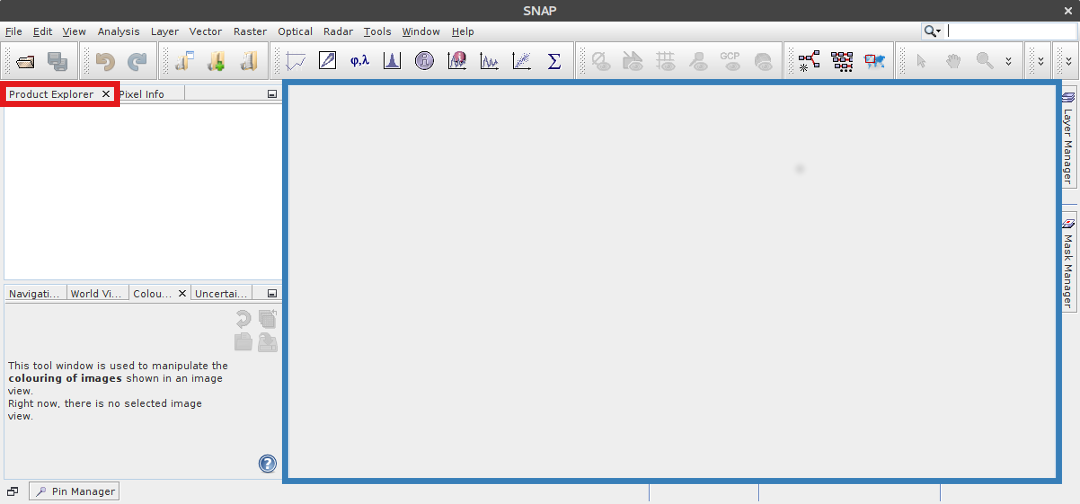
\includegraphics[width=0.7\textwidth]{fig:int.png}
    \caption{Interfaz gráfica del usuario. El área de visualización -en azul- con el \menu{Product Explorer} a la izquierda -en rojo-.}
    \label{fig:int}
\end{figure}

\section{Apertura de imágenes}

Desde el menú \menu{File>Open product...} abra la imagen óptica
\begin{center} \directory{raster\_data/S2A\_USER\_MTD\_SAFL2A\_PDMC\_20161206.dim}.
\end{center}
Haga doble click sobre el nombre de la imágen y se desplegará, en el \menu{Product Explorer} un árbol que incluye:
\\
\dirtree{%
    .1 [1] S2A\_USER\_MTD\_SAFL2A\_PDMC\_20161206.
    .2 Metadata.
    .2 Vector Data.
    .2 Bands.
    .2 Masks.
}

En esta cobertura encontramos

\begin{itemize}
    \item \emph{[1] S2A\_USER\_MTD\_SAFL2A\_PDMC\_20161206}: El número de elemento entre corchetes, que marca en que orden se abrieron los productos y el nombre de la imagen.
    \item \emph{Metadata}: Los metadatos asociados a la imagen y su historial de procesamiento.
    \item \emph{Index Codings}: Los valores de referencia para interpretar los números digitales de la imagen.
    \item \emph{Bands}: Las bandas de la imagen y las operaciones de álgebra entre bandas.
    \item \emph{Masks}: Las mascaras de la imagen y si las hubiera.
\end{itemize}

\section{Visualización}

Para visualizar una de las bandas de la imagen haga doble click sobre el nombre y se mostrará en escala de grises (Figura \ref{fig:mono}). Es posible abrir varias bandas en simultáneo, cada una se mostrará en una pestaña nueva arriba del área de visualización. Explore la imagen utilizando las herramientas de navegación y zoom (Figura \ref{fig:mono})

\begin{figure}[h!]
    \centering
    \subfloat[]{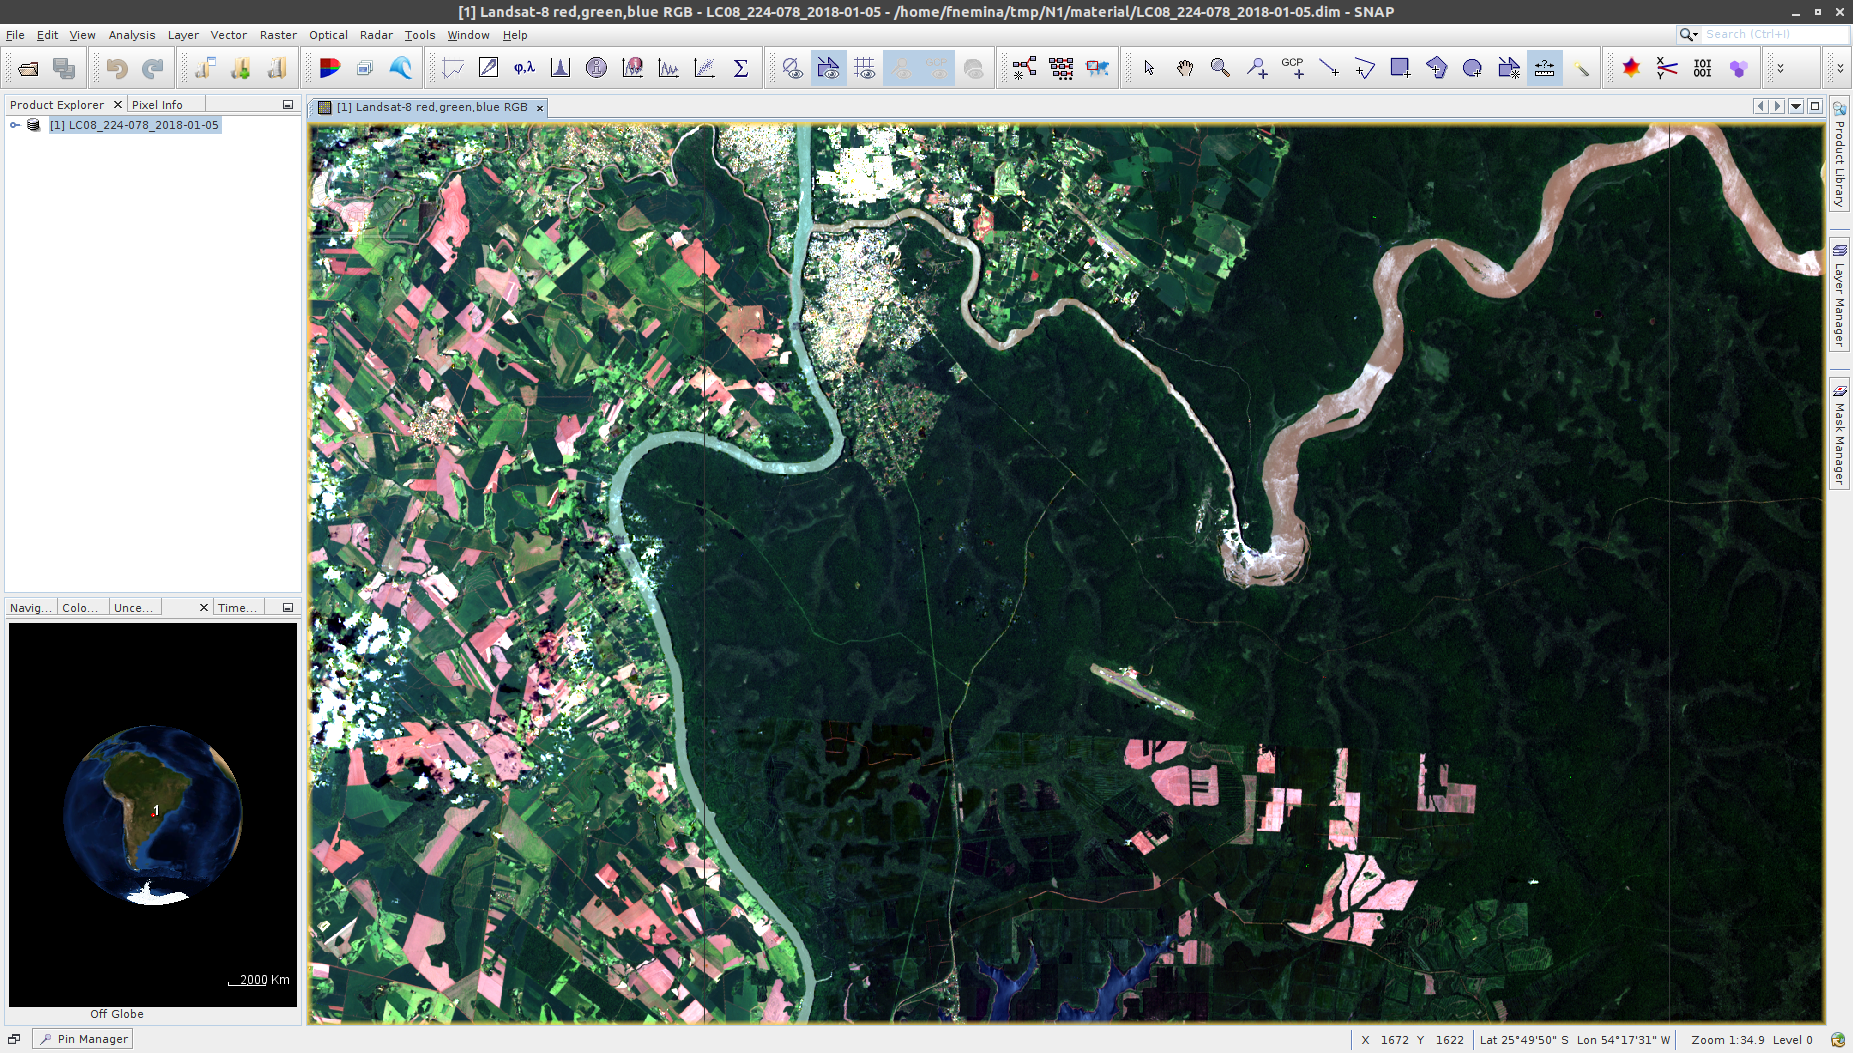
\includegraphics[width=0.7\textwidth]{fig:mono.png}}
    \\
    \subfloat[]{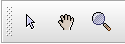
\includegraphics[scale=0.5]{fig:NAV.png}}
    \caption{Imagen monobanda desplegada en el visualizador. Herramientas de navegación. De izquierda a derecha: \menu{Selection tool}, para seleccionar objetos, \menu{Panning tool}, para moverse, y \menu{Zooming tool}, para hacer zoom.}
    \label{fig:mono}
\end{figure}


En el \menu{Product Explorer} seleccione \menu{Open RGB image windows} haciendo click derecho sobre el nombre de la imagen. Se desplegará una nueva ventana (Figura \ref{fig:RGB}) que le permitirá elegir la combinación de bandas. Por defecto aparecerá la combinación que utiliza las bandas 4, 3 y 2 de Sentinel 2, desplieguela haciendo click en OK.

\begin{figure}[h!]
    \centering
    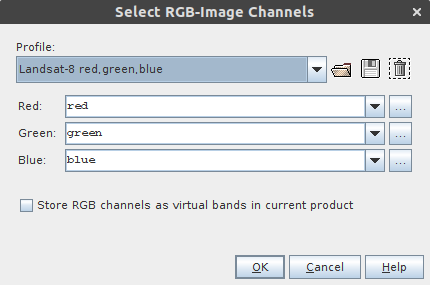
\includegraphics[scale=0.7]{fig:RGB.png}
    \caption{Ventana de combinación de bandas. Puede eligir una banda para cada canal del monitor (\emph{Red, Green, Blue}) o puede optar por una preseleccionada del menú \emph{Profile}}
    \label{fig:RGB}
\end{figure}


\section{Consulta de píxel}

Para obtener información sobre un pixel seleccione la pestaña \menu{Pixel info}, junto al \menu{Product explorer} (Figura \ref{fig:pixel}), y posicionese  sobre uno en la imagen.

\begin{figure}[h!]
    \centering
    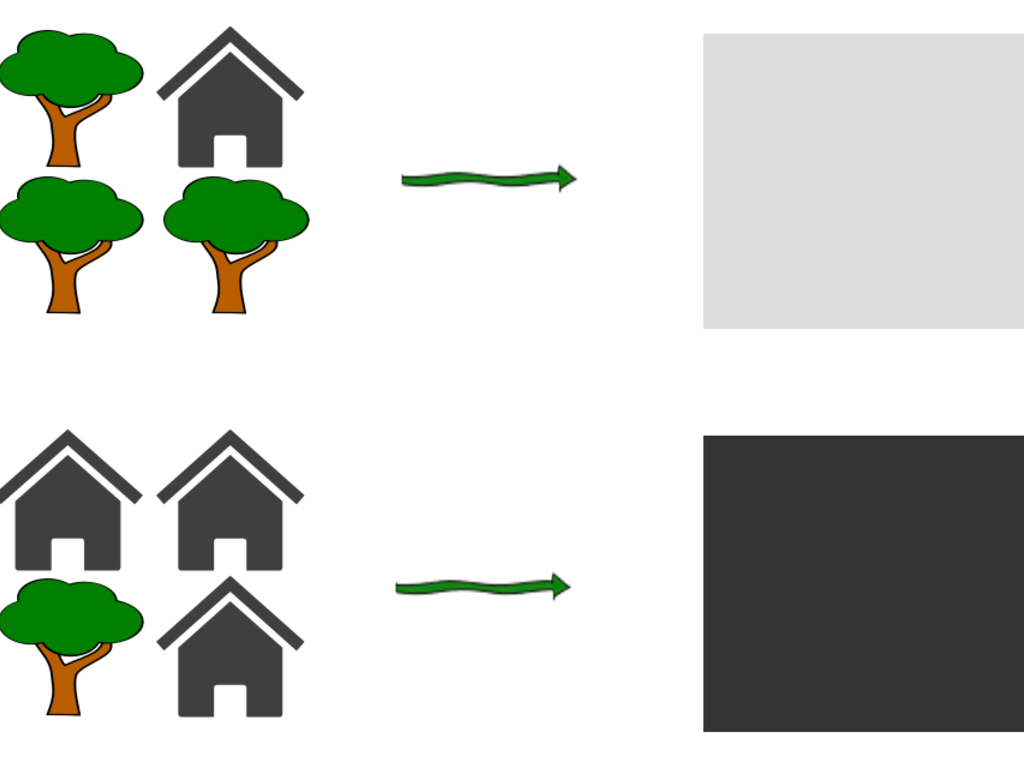
\includegraphics[width=0.3\textwidth]{fig:pixel.png}
    \caption{Herramienta de consulta de píxel. Puede verse la posición del píxel en la imagen, su latitud y longitud y el valor del píxel para la banda desplegada.}
    \label{fig:pixel}
\end{figure}

Allí encontrará la latitud y longitud, las coordenadas dentro del mapa y el valor del pixel en la banda abierta.

\section{Exportar pantalla}

Es posible exportar la visualización de la imagen completa o de una región específica desde \menu{File>Export>Other}.
Si selecciona \menu{View as image} generará archivos \texttt{.GeoTiff} o \texttt{.jpg} para visualizarlo en otro software. Para mantener la georreferencia debe optar por \texttt{GeoTIFF - TIFF with geo-location} con la opción \texttt{Full resolution}. De esta manera se mantiene la resolución original de la imagen (Figura \ref{fig:export}).

\begin{figure}[h!]
    \centering
    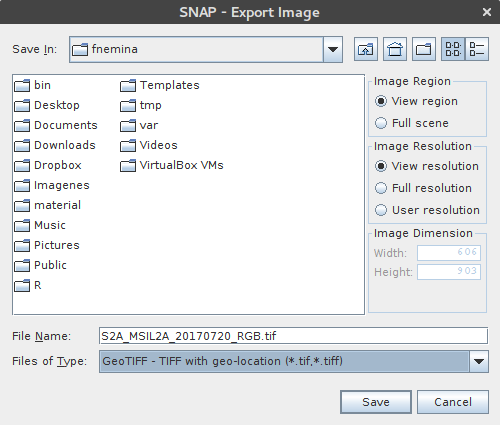
\includegraphics[width=0.4\textwidth]{fig:export.png}
    \caption{Menú de \menu{Export image}. Incluye las opciones para elegir el recorte, la resolución y el tipo de dato de salida.}
    \label{fig:export}
\end{figure}

Si selecciona \menu{View as Google Earth KMZ} obtendrá un archivo \directory{.kmz} que luego podrá abrir desde Google Earth (Apéndice \ref{ap:GE}).

\section{Preguntas para debate}

Abra la imagen radar correspondiente al satélite \emph{COSMO-SKYMED} que se encuentra en
\begin{center}
\directory{raster\_data/CSKS1\_SCS\_B\_S2\_04\_HH\_RA\_FF\_20090321.dim}
\end{center}
Abra la banda \texttt{Sigma0\_HH\_db}.

\begin{que}
    Identifique en la imagen zonas brillantes u oscuras. ¿A que cobertura pertenecen?
\end{que}

\begin{que}
    ¿Cómo es el nivel de brillo para los cuerpos de agua?
\end{que}

\begin{que}
    ¿Cuales son las coordenadas aproximadas del aeropuerto que se encuentra en el centro de la imagen?
\end{que}

Estas preguntas no serán evaluadas. Su objetivo es discutirlas en el foro de sonsultas e intercambio de la clase.
